\insertmeeting 
	{Beginning-of-Season Outreach Planning} 
	{08/30/22}
	{Hagerty High School}
	{Jensen, Jorge, Karissa, Laura, Samantha, Tyler}
	{Images/RobotPics/robot.jpg}
	{2:30 - 4:00}
	
\hhscommittee{General}
\noindent\hfil\rule{\textwidth}{.4pt}\hfil
\subsubsection*{Goals}
\begin{itemize}
    \item Propose new outreach ideas

\end{itemize} 

\noindent\hfil\rule{\textwidth}{.4pt}\hfil

\subsubsection*{Accomplishments}
We began by looking at the past Outreach opportunities that had been come up with before. During the past season we had already come up with an extensive list, including Programming/OnShape/Photoshop tutorials, demoing robots at FLL events/for sponsors, and donating shoes or socks for the poor. These were considered on top of our usual FLL mentoring, which preparation for was already put in motion for, as well as our contributions to Operation Paperback, which collects book donations to send to military families. We didn't confirm anything in particular in terms of past items, but it was still good to go back over them to keep these still good ideas in mind. 
Once we reviewed old ideas, it was time to think of new ones. We drew some inspiration from the theme for this FIRST season: Energize. This season is all about promoting clean energy, and discussing how we will power the technology that drive our lives, including FIRST itself. From that, we got ideas like touring power plants, promoting our school board to put their public schools on solar, and collecting used batteries so they can be disposed of properly.
Of course, there are more outreach ideas to think of than those related to the season; we have connections with the mayor, as during the previous season we talked to her about our program. From that, we got the idea to contact her to organize a robotics day with all of our local teams in Oviedo on the Park, a local public social center where many events are organized. In doing this, we could spread FIRST far further than we could without the cooperation of our local teams and mayor. We also had the idea to adopt a park, that way as a program, we can help maintain the environment of our local community.
Overall, we didn't decide too much of a concrete plan in terms of Outreach, but this meeting was still very important for planning Outreach in the future, and is going to influence our actions significantly going forward.


% \begin{figure}[htp]
% \centering
% 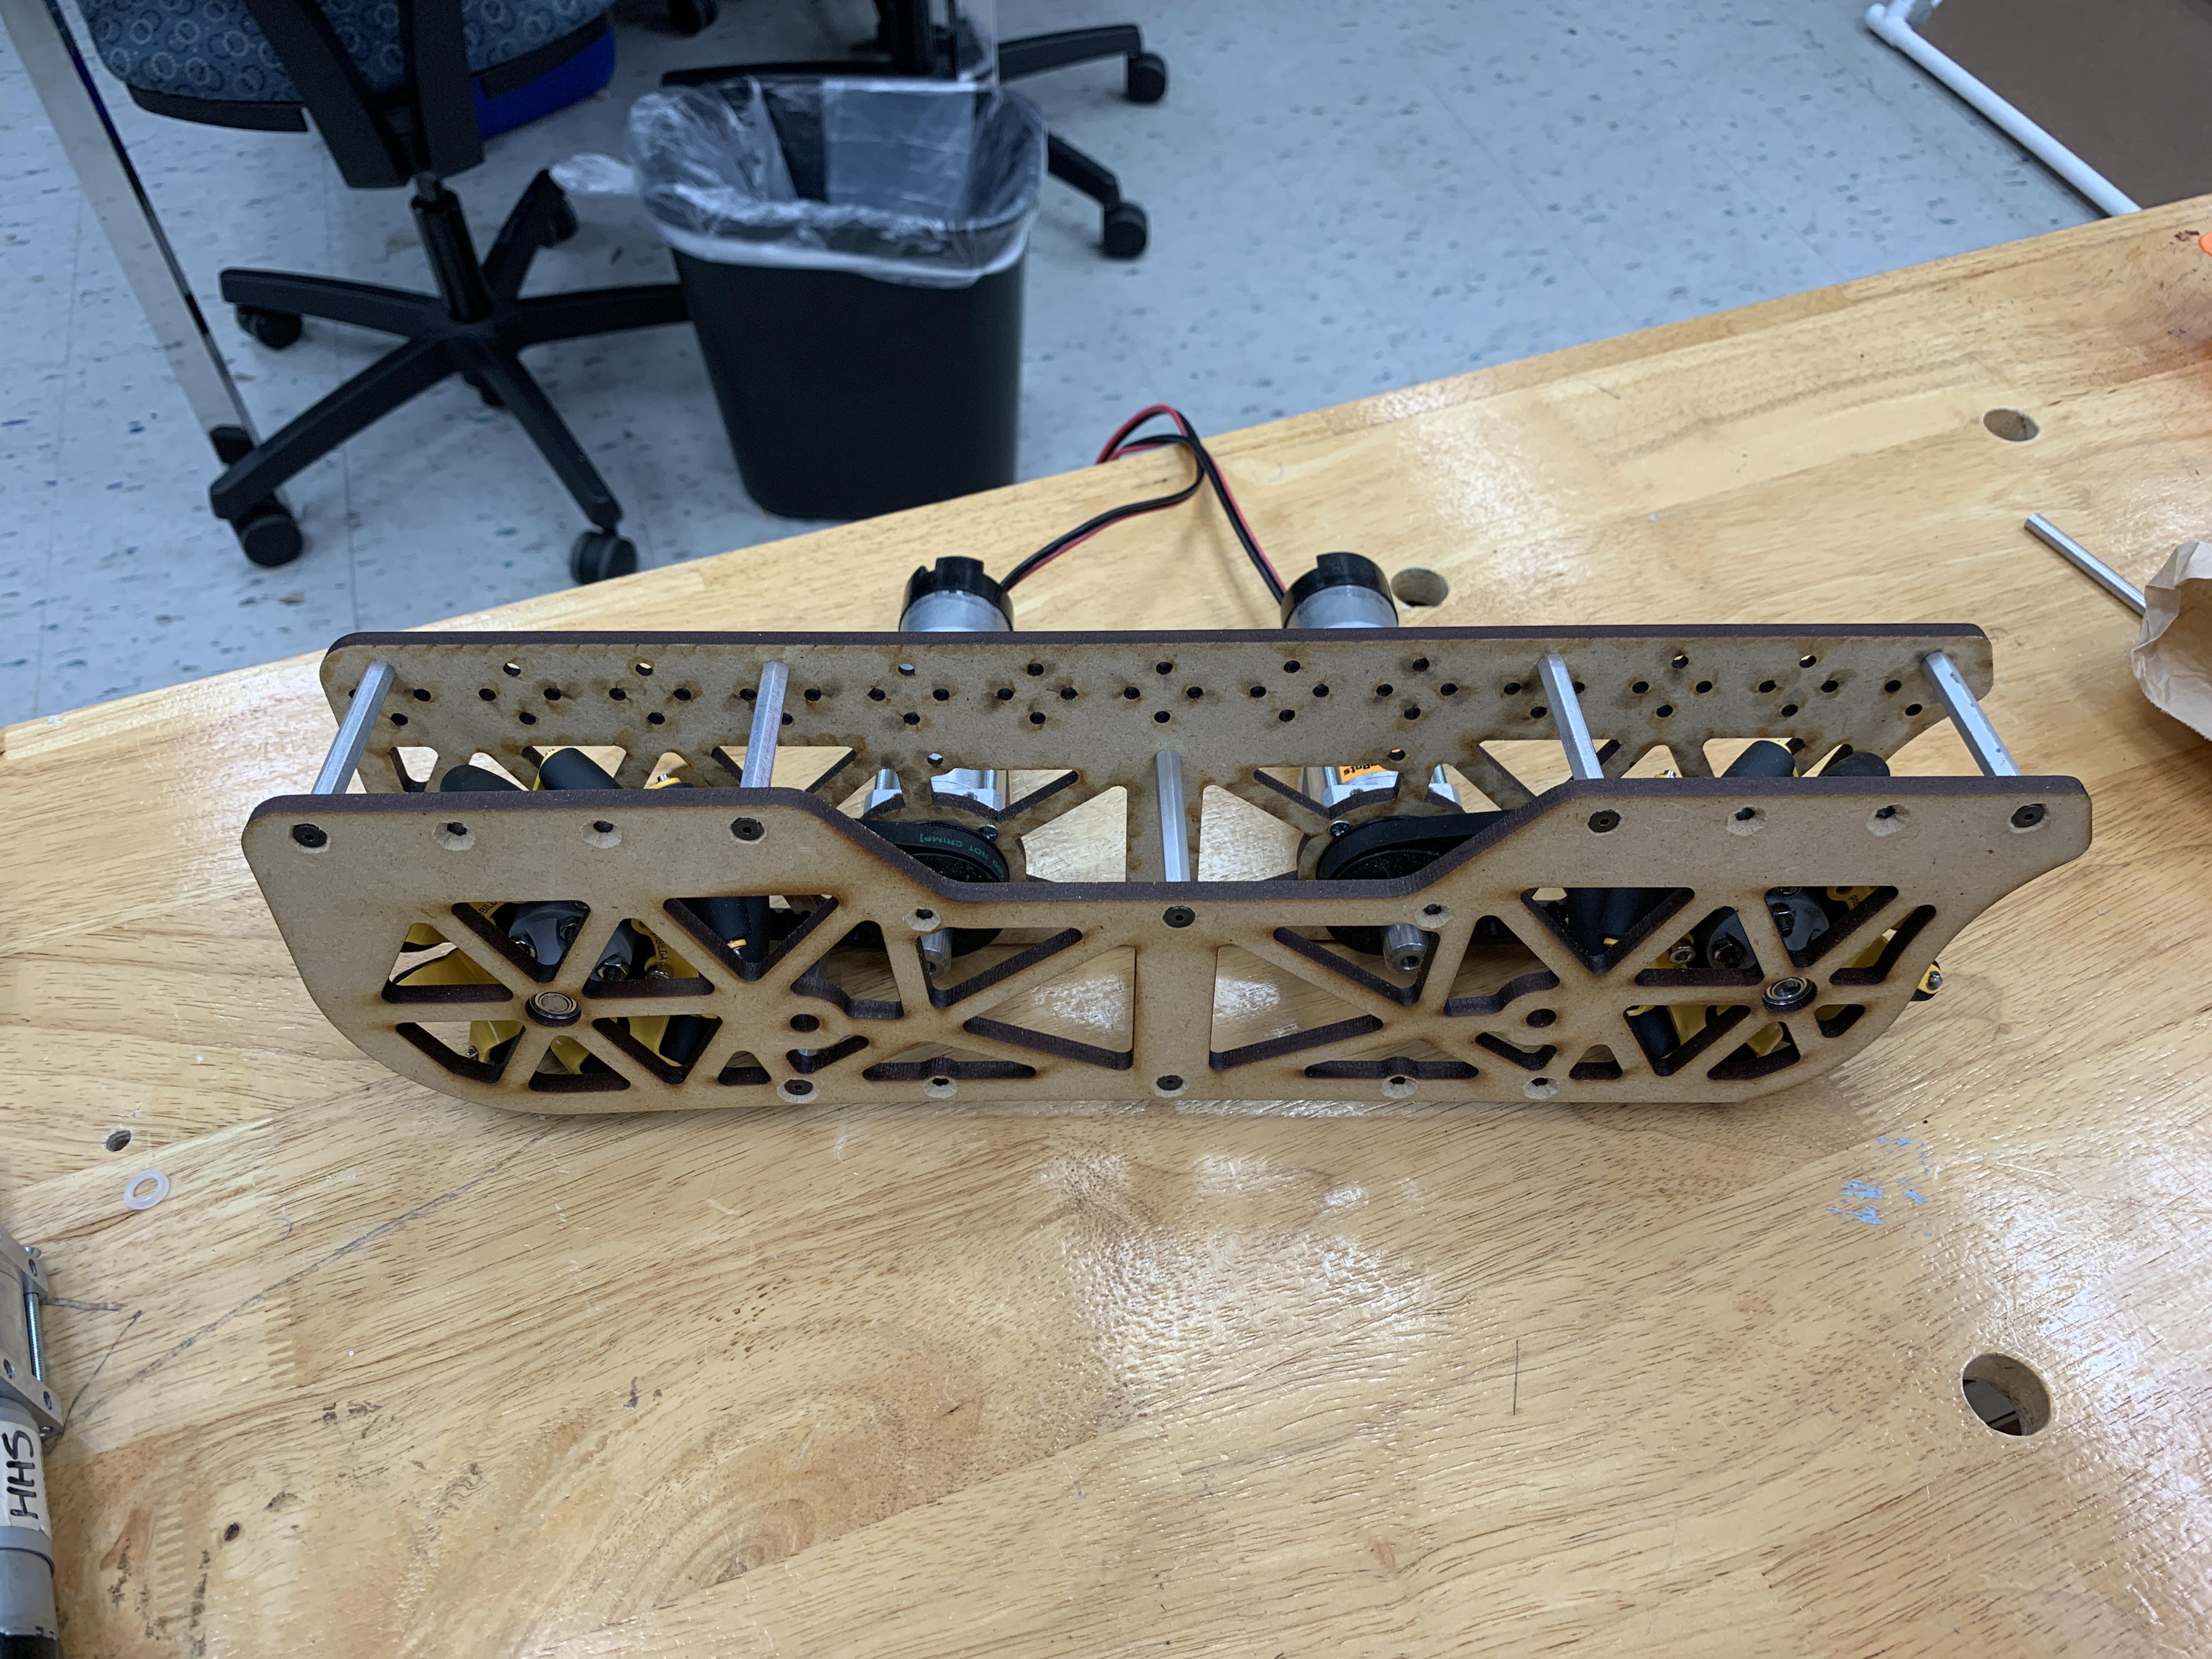
\includegraphics[width=0.9\textwidth, angle=0]{Meetings/July/07-21-21/drivetrain_7-20-21-NathanForrer.jpg}
% \caption{First half of the drivetrain.}
% \label{fig:072121_1}
% \end{figure}

\whatsnext{
\begin{itemize}
    \item Update team website
	\item - Kick-start social media to start the season
\end{itemize} 
}
